\documentclass[output=paper]{LSP/langsci}  
\author{Martijn Wieling\affiliation{University of Groningen, CLCG} \lastand  Simonetta Montemagni\affiliation{Istituto di Linguistica Computazionale “Antonio Zampolli”, ILC-CNR}} 
\title{Infrequent forms: Noise or not?}
\abstract{In this study we ask the question whether simplifying the data in dialectometrical studies by removing infrequent forms is advantageous to 
%original: uncover 
uncovering the geographical structure in dialect data. By investigating lexical variation in a large corpus of Tuscan dialect data via hierarchical bipartite spectral graph partitioning, we are able to identify the main geographical areas together with their linguistic basis. In order to assess the influence of infrequent forms, we conduct two analyses: one which includes only lexical variants used by at least 0.5\% of the informants, and another which includes all lexical variants in the data. Using this approach we show that using all data enables us to find a geographical characterization with a more adequate linguistic basis than by using the trimmed data.
}

\maketitle 
\begin{document}
  

% {\centering Infrequent forms: Noise or not?\\
% \vskip11pt
% \begin{multicols}{2}
% \centering \\
% \centering University of Groningen, CLCG\\
% \vskip11pt
% \centering\\
% \centering CNR, Istituto di Linguistica Computationale ‘Antonio Zampolli’\\
% \end{multicols}}
 

\section{Introduction}
Dialectometry (\citealt{seguy_relation_1971}; see \citealt{wieling_advances_2015} for an overview) proceeds from the idea that aggregating over a large set of linguistic items will yield a better view of dialectal variation than subjectively selecting a few linguistic items \citep[190--191]{nerbonne_data-driven_2009}.  In quantitative linguistics, it is generally noted that infrequent words constitute noise, and are unreliable evidence of linguistic structure \citep[199]{manning_foundations_1999}. With respect to lexical differences in dialectology, this view is supported by \citet[17]{carver_american_1987}. In contrast to this, however, stands the opinion of \citet[Vol I: 83--86]{goebl_dialektometrische_1984}, who argues that infrequent words (i.e. word forms used by only a few informants) should be considered more informative (i.e. weighted more) when determining the strength of the linguistic relationship between two sites.

Supporting Goebl's (\citeyear{goebl_dialektometrische_1984}) view, \citet{nerbonne_toward_2007} show that removing infrequent words results in less adequate linguistic distances than including all data. \citet[173]{kretzschmar_scaled_2013} are also in favor of including infrequent elements and argue that ``[methods in dialectology which only notice the few most frequently occurring variants and ignore the rest] cannot address the underlying complexity of the data.''

At present, however, many researchers in dialectometry still ignore infrequent items under the presumption that these are noise. For example, \citet{wieling_analyzing_2014} only use the top-ten most frequent variants for each concept in a study on English lexical variation, and \citet{szmrecsanyi_corpus-based_2011} ignore infrequent items in a morpho-syntactic dialectometric study. 

We believe that the contrasting views reported above are based on two different notions of word frequency, namely that of token and type frequency. Whereas \citet{manning_foundations_1999} refer to a notion of token frequency (i.e. counting how often a particular form appears in the input), frequency based on dialectal data gathered through questionnaires should be interpreted as type frequency (i.e.  the number of distinct lexical items that can be substituted to express the same meaning). \citet{bybee_phonology_2001} argues that type rather than token frequency underlies productivity, the diachronic consequence of which may be lexical enrichment. Following this line of reasoning, from a diatopic perspective we can hypothesize that type frequency is related  to lexical variation. The question we started with can therefore be reformulated as follows: What is the role and impact of lexical type frequency in dialectometrical studies based on atlas data in uncovering the geographical structure underlying them? To answer this question, we will evaluate the effect of taking into account all data, versus ignoring lexical variants used in at least two locations by 10 informants or fewer (out of a total of 2060 informants).

\section{Data}
In this study, we investigate Tuscan lexical variation on the basis of the \textit{Atlante Lessicale Toscano} (ALT, \citealt{giacomelli_atlante_2000}), available as an online resource (\url{http://serverdbt.ilc.cnr.it/ALTWEB}). The dialect data used in this study contains the results gathered in response to 170 onomasiological questions, i.e. starting from concepts and looking for their lexicalizations, in 213 locations. In each location, multiple informants were interviewed of varying age. Consequently, a total of 2060 informants are included in this dataset. \citet{montemagni_tracking_2015} provides an extensive overview of this data source. In short, the dataset consists of noun concepts only, which resulted in at most 50 different (normalized) lexical variants, and responses were normalized to abstract away from phonetic variation. This dataset has also been used by \citet{wieling_lexical_2014} to investigate lexical variation in Tuscany with respect to standard Italian. While our approach is also applicable to other types of linguistic data (such as phonetic, syntactic or morphological data), the large number of informants behind this dataset ensure low frequent variants can be reliably identified.

\section{Methods}
We analyze the dataset using hierarchical bipartite spectral graph partitioning (HBSGP; \citealt{wieling_bipartite_2011}). This advanced clustering approach simultaneously clusters the geographic locations together with the linguistic variants, thereby yielding a linguistic basis of the geographical clustering. In short, the method functions by constructing a bipartite graph, which is a graph consisting of two sets of vertices. One set of vertices represents the locations, whereas the other set represents the lexical realizations of the 170 investigated concepts or, in short, lexical variants. Whenever a lexical variant is used in a location, there is an edge between the variant and the location. The width of the edge represents the proportion of informants in a location using the variant. There are no edges between pairs of locations or pairs of variants. The HBSGP  algorithm determines which edges to cut in such a way that as few (thick) edges as possible are cut to obtain two separate bipartite graphs (i.e. the two graphs are not connected) and the number of vertices in both graphs is (approximately) balanced. Consequently, the two new bipartite graphs represent two clusters in which lexical variants are grouped together with the locations they are most strongly associated with. The optimal clustering is determined via the singular value decomposition of a (normalized) matrix representation of the original bipartite graph, which is subsequently subjected to the \textit{k}{}-means clustering algorithm (with \textit{k} = 2) to determine the two-way clustering. The hierarchical clustering is obtained by recursively applying the HBSGP algorithm to the separate bipartite graphs. A more detailed explanation of the method and the mathematical details can be found in \citet{wieling_bipartite_2011}. Besides having been applied to pronunciation variation (e.g., \citealt{wieling_bipartite_2011}), HBSGP has been previously applied to analyze English lexical variation \citep{wieling_analyzing_2014}. 

To identify the most important linguistic variants, two measures have been proposed by \citet{wieling_bipartite_2011}: representativeness and distinctiveness. Representativeness of a variant in a cluster is defined as the relative frequency of the variant in the cluster. In each location the relative frequency of the variant ranges between 0 (no informant uses the variant) and 1 (all informants use the variant). By summing these relative frequencies for all locations in the cluster and dividing this value by the number of locations in the cluster, the representativeness is obtained. Consequently, a representativeness of 0 indicates that the variant is not used in any of the locations in the cluster, while a representativeness of 1 indicates that all informants in all locations in the cluster use the variant. 

Distinctiveness measures how frequent the variant occurs within as opposed to outside of the cluster. It also takes the relative size (i.e. the number of locations) of the cluster into account to correct for chance effects. Consequently, distinctiveness requires two values, the relative occurrence of the variant in the cluster and the relative size of the cluster. The relative size is calculated by dividing the number of locations in the cluster by the total number of locations in the dataset. The relative occurrence is calculated by summing the relative frequencies of the variant for all locations in the cluster (as was done for representativeness) and dividing this number by the summed relative frequencies of the variant in all locations in the dataset. Subsequently, distinctiveness is calculated by subtracting the relative size from the relative occurrence and dividing this value by the relative size subtracted from 1. A distinctiveness of 1 indicates that the variant is only used within the cluster, and not outside the cluster, whereas a distinctiveness of 0 (or lower) indicates that the variant is used equally (or less) frequently as would be expected on the basis of the relative size of the cluster. For example, if the relative occurrence is 0.75, and the relative size is 0.25, the distinctiveness is equal to $\frac{0.75 - 0.25}{1 - 0.25} = 0.67$.

In previous studies (e.g., \citealt{wieling_analyzing_2014}) the importance of a variant has been determined by taking the mean of representativeness and distinctiveness, but here we follow the approach of \citet{montemagni_tracking_2015} in multiplying the two values (i.e. importance = distinctiveness x representativeness).

In the following, we will evaluate the choice of taking into account all lexical data (``full'') versus ignoring variants used by at most 0.5\% of the informants (``trimmed'': ignoring variants used by 10 or fewer informants out of all 2060 informants) by investigating the importance values of the most characteristic variants associated with the various clusters. The underlying idea is that a better clustering will be characterized by more distinctive and representative linguistic variants. \figref{fig:1} visualizes the typical frequency distribution of the lexical variants associated with a specific concept (i.e. showing the number of informants using each variant, in this case of the concept \textit{susina}, `plum') and the red dots indicate the low-frequency variants (i.e. those used by a maximum of 10 informants) excluded in the trimmed dataset.

\begin{figure}
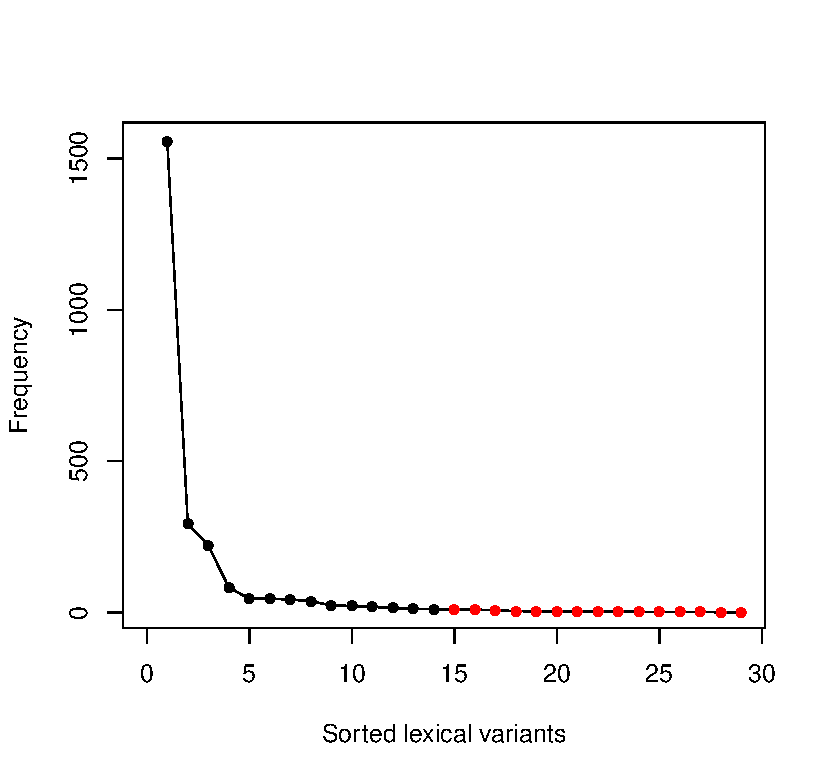
\includegraphics[width=.75\textwidth]{illustrations/wiel_monte_fig1}
\caption{Number of informants in the different locations (i.e. type frequency) using the various lexical variants for the concept `plum'. The red dots indicate the variants excluded in the trimmed dataset. The variants are sorted by decreasing frequency.}
\label{fig:1}
\end{figure}

\begin{figure}
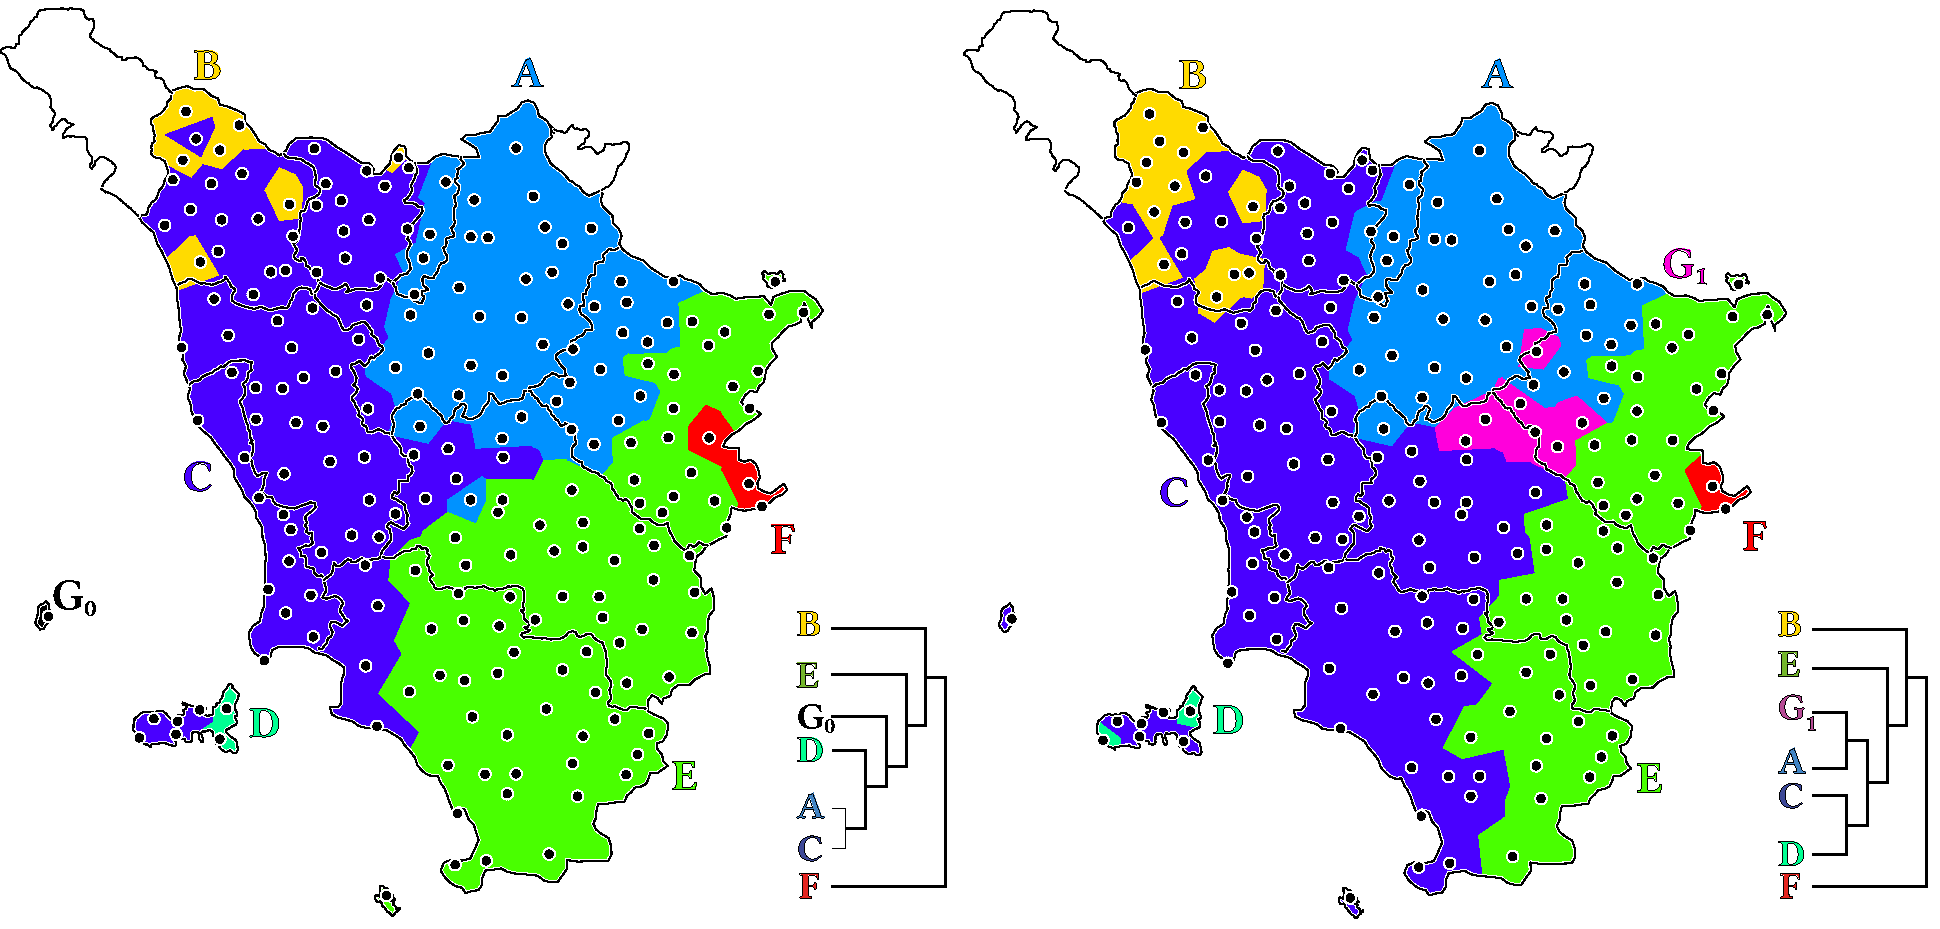
\includegraphics[width=\textwidth]{illustrations/wiel_monte_fig2}
\caption{Clustering of Tuscan dialects in seven groups. Left: based on full dataset. Right: based on trimmed dataset.}
\label{fig:2}
\end{figure}

\begin{figure}
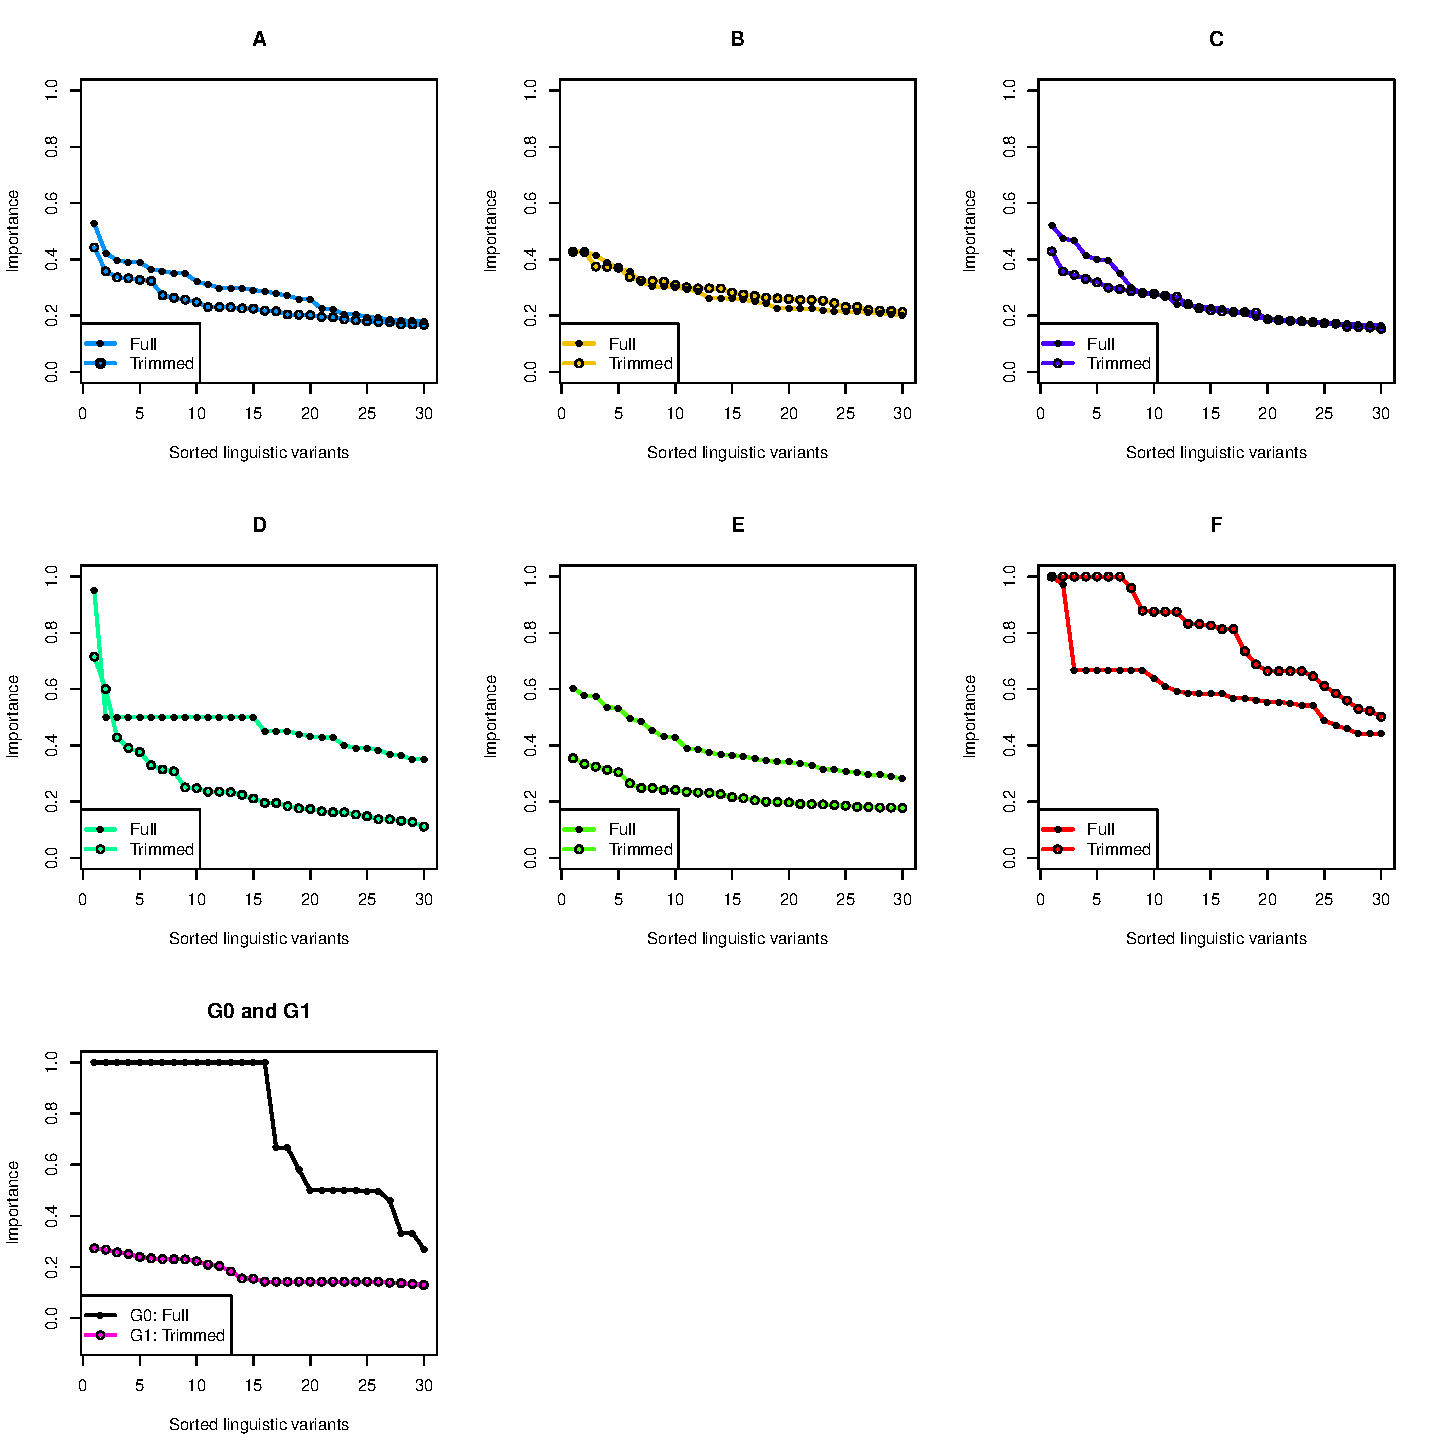
\includegraphics[width=\textwidth]{illustrations/wiel_monte_fig3}
\caption{Sorted importance values for each of the seven groups. The solid dots are associated with the full dataset while the open dots are associated with the trimmed dataset. The line color matches the color of the groups in \figref{fig:2}.}
\label{fig:3}
\end{figure}

\section{Results}
\figref{fig:2} shows two cluster maps (seven groups) on the basis of both datasets. \figref{fig:3} shows the top-thirty importance values associated with the most relevant lexical variants for each of the seven groups on the basis of the two datasets. The importance values were calculated for all variants available per dataset (i.e. all 5174 variants for the complete dataset, and the 1996 variants having a frequency of at least 11 for the trimmed dataset). Only the top-thirty variants are visualized, as the number of associated variants per cluster varied. Clearly, the results on the basis of the full dataset (solid dots) are generally more reliable than those on the basis of the trimmed dataset (open dots). Especially the large clusters (A, C and E) appear to be better characterized on the basis of the full data. For the smaller clusters the results appear to be more mixed. However, when averaging the top-three importance values across the seven groups, the mean importance score for the full dataset is 0.639, whereas it is only 0.478 for the trimmed dataset. This pattern remains similar when looking at the top-ten (0.560 vs. 0.413) or top-thirty variants (0.435 vs. 0.316), and also holds when specifically focusing on distinctiveness (top-three: 0.997 vs. 0.981, top-ten: 0.971 vs. 0.912, top-thirty: 0.881 vs. 0.745) or representativeness (top-three: 0.891 vs. 0.867, top-ten: 0.777 vs. 0.754, top-thirty: 0.630 vs. 0.591). Clearly, taking into account infrequent items helps to improve results on the basis of the HBSGP method. Given that this method takes as input individual variants and their relative frequency in each location, the full dataset obviously contains much more information.  By contrast, when calculating distances on the basis of these lexical variants (i.e. by using the matrix representation of the bipartite graph as input for the online dialectometry application Gabmap; \citealt{nerbonne_gabmap_2011}), the distance matrices on the basis of both datasets have a correlation of \textit{r} = 0.81. Furthermore, \figref{fig:4} shows that the clustering (7 clusters, on the basis of Ward's method) is hardly affected at all.

\begin{figure}
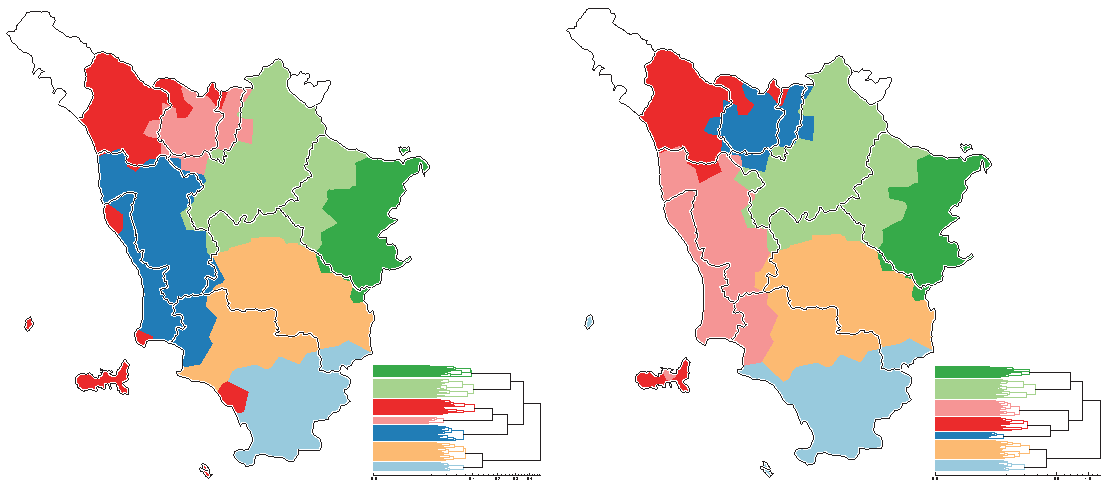
\includegraphics[width=\textwidth]{illustrations/wiel_monte_fig4}
\caption{Distance-based clustering of Tuscan dialects in seven groups using Ward's method. Left: based on full dataset. Right: based on trimmed dataset.}
\label{fig:4}
\end{figure}

\section{Discussion}
In this study we have shown that cluster quality improves when the analysis is based on all data, rather than using a subset in which infrequent variants are filtered out. This effect appears to be greater for a feature-based clustering method, such as hierarchical bipartite spectral graph partitioning, than for distance-based clustering, where the influence is only limited. In the case of the HBSGP method, the improvement is observed at the level of both the clustering of locations into dialectal areas and the identification of the most important associated lexical variants. These findings support and extend earlier findings of \citet{nerbonne_toward_2007} and suggest that investigating geographical patterns of dialect variation on the basis of all data might be a worthwhile approach when studying dialects in the future. Further studies on the role of type frequency in dialectometry might investigate whether and to what extent it relates with productivity,  to be interpreted here as geographic lexical variability.

\printbibliography[heading=subbibliography,notkeyword=this]
\end{document}